Before comparing the map to anything, it is worth looking at what the curator
built, because its shape is not the shape one might expect from a taxonomy.

\paragraph{It is a map of support, not of division.}
The \NAssertions{} assertions fall into ten relation types, and two of them
account for more than half: \rel{supports} (\RelSupports{}) and
\rel{requires} (\RelRequires{}). Relations that separate ideas are a distinct
minority: \rel{opposes} (\RelOpposes{}) and \rel{contrasts\_with}
(\RelContrastsWith{}) together are barely a fifth of the total. The map says
far more about what holds up what than about what rules out what.

\paragraph{It says more than one thing about the same pair.}
Those \NAssertions{} assertions cover only \NPairs{} distinct pairs of
concepts, \AssertionsPerPair{} per pair. \PairsMulti{} pairs carry more than
one assertion and \PairsConflicting{} carry assertions of different kinds.
Some of these are complementary --- \rel{requires} together with
\rel{supports} is the commonest combination --- but others encode a real
tension the curator declined to resolve, such as the nine pairs marked both
\rel{contrasts\_with} and \rel{supports}, or the five marked both
\rel{opposes} and \rel{requires}. A concept pair that opposes and requires at
once is not a modelling error; it is an accurate report of a literature in
which self-love and benevolence are set against each other on one page and
made to need each other on the next.

\paragraph{It ignores its own categories.}
Each concept sits in a three-level category tree whose top level has nine
branches, the largest being Ethics (48 concepts), Moral Psychology (36),
Theology (30) and Metaphysics (30). If the categories organised the map, edges
would mostly stay inside them. They do not: \CrossCategoryPct\% of edges cross
a top-level boundary, the commonest crossings being Ethics to Moral Psychology
(84 edges) and Ethics to Theology (54). Community detection recovers
\NCommunities{} groups at modularity \Modularity{}, which is real structure
but not the category tree; the groups cut across it.

\paragraph{Its hubs are old words.}
\TopHub{} is the most connected concept by a wide margin
(\TopHubDegree{} neighbours), followed by Liberty (60), Reason (51), Habit
(49) and Providence (49). The same five top the betweenness ranking, so they
are not merely popular but load-bearing: remove them and the map falls into
pieces. What is notable is which words these are. None of the terms that
period scholarship treats as the distinctive contribution of the century ---
moral sense, sympathy, the impartial spectator --- appears near the top.
The map's skeleton is the vocabulary the century inherited, not the
vocabulary it invented.

\begin{figure}[t]
  \centering
  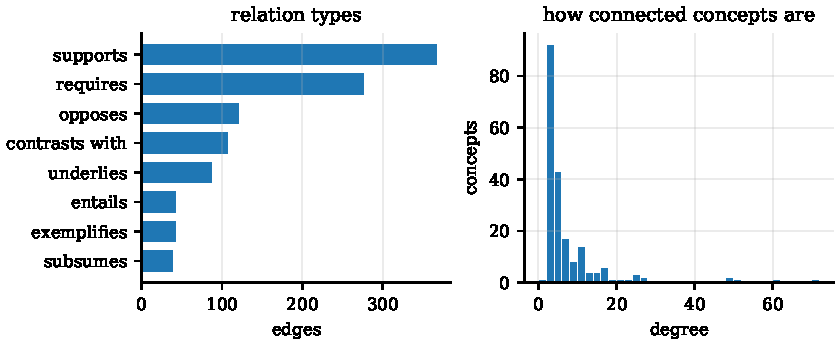
\includegraphics[width=\linewidth]{graph_anatomy.pdf}
  \caption{Left: the relation types the curator reached for, dominated by
           \rel{supports} and \rel{requires}. Right: how connected concepts
           are. The distribution is heavily skewed --- most concepts have a
           handful of neighbours and a few have dozens.}
  \label{fig:graph}
\end{figure}

\paragraph{Connection follows the books, not the curator's judgement.}
Each concept carries two curator-assigned numbers: an \emph{importance} score
and a \emph{book count} recording how many works it was found in. Degree in
the finished graph correlates strongly with book count
($\rho=\RhoBookCount{}$) and only weakly with importance
($\rho=\RhoImportance{}$). Whatever the curator meant by importance, it is not
what determined how the map got wired; textual spread is. This matters for the
next section, because it means the map is already, in part, a record of
distributional facts --- which makes the places where it \emph{departs} from
the distributional record the interesting ones.
